\documentclass{article}
\usepackage{parskip}
\usepackage{geometry}
\usepackage{graphicx}
\addtolength{\oddsidemargin}{-.875in}
\addtolength{\evensidemargin}{-.875in}
\addtolength{\textwidth}{1.75in}

\addtolength{\topmargin}{-.875in}
\addtolength{\textheight}{1.75in}
\begin{document}

\begin{center}
	\fontsize{22pt}{1.2}\textbf{\vspace{10px} Orbit Reference}\\
	\large\today\vspace{30px}
\end{center}


This is a quick reference of various useful equations relating to astrodynamics.

\section{Ellipse}

An ellipse is defined as a circular shape with two axes of freedom, the long axis is called the major axis, the shorter axis is the minor axes, the difference in length of the major and minor axes determines the eccentricity.

Eccentricity $\varepsilon$ ranges from greater than zero to less than 1 for an ellipse, zero is a circle, one is a parabola, greater than one is a hyperbola.

The equation for an ellipse in polar coordinates is:

$r = \frac{a(1-\varepsilon^2)}{1+\varepsilon \cos \theta}$

An alternative is:

$r = \frac{\ell^2}{m^2\mu} \frac{1}{1+\varepsilon \cos\theta}$ where $\ell = mvr$ and $\mu = GM $

Note: distance and velocity should be from the periapsis.

\subsection{Conversion to rectangular coordinates}

The equation to convert from polar to rectangular is:

$ x = r \cos \theta\\y = r \sin \theta $

\subsection{Distance from centre}

The minimum and maximum distance from the centre of orbit to the centre of the body (pericentre and apocentre) can be calculated with:

$ r_{min} = \frac{a(1-\varepsilon^2)}{1+\varepsilon} $\\[5px]
$ r_{max} = \frac{a(1-\varepsilon^2)}{1-\varepsilon} $

The same applies to the alternative equation, just drop the cosine $\theta$.

\subsection{Apoapsis and Periapsis}

The apocentre and pericentre distance can be converted to apoapsis and periapsis (from centre of orbit to surface of body) by adding the radius of the body.

\subsection{Semi-major axis}

Semi-major axis (half the major axis length) can be calculated from the apocentre and pericentre distance:

$ a = \frac{r_{min} r_{max}} {2} $

\subsection{Semi-minor axis}

The semi-minor axis (half the minor axis length) can be calculated with:

$ b = \sqrt{r_{min} r_{max}} $

\subsection{Linear eccentricity}

Linear eccentricity is the distance between centre of the ellipse and the focal point:

$c = \sqrt{a^2 - b^2} $

\subsection{Eccentricity}

The eccentricity of an ellipse is:

$ \frac{c}{a} $ or $ \sqrt{1- \frac{b^2}{a^2}} $ or $ \frac{ApC-PeC}{ApC+PeC} $

\subsection{Semi-latus rectum}

The semi-latus rectum which is the line at a right angle to the focus is:

$ \ell = \frac{b^2}{a} $ or $ a (1-\varepsilon^2) $

\begin{figure}[h]
	\centering
	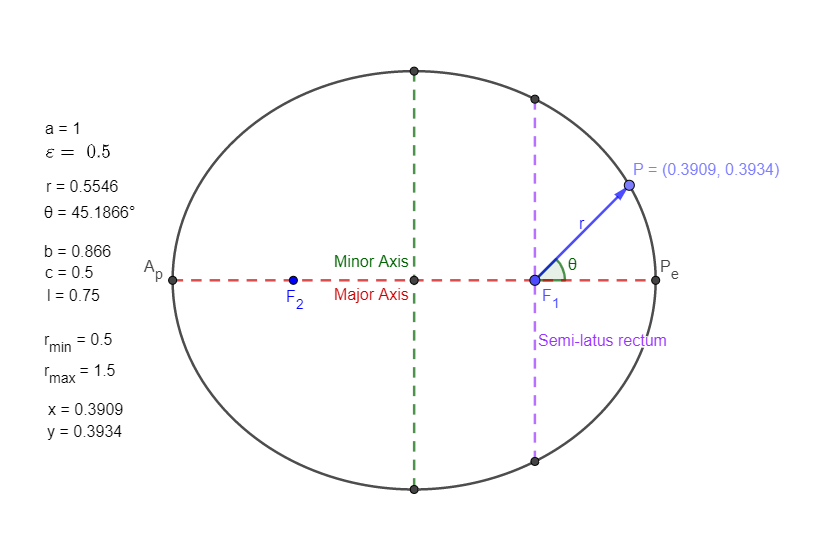
\includegraphics[width=0.9\linewidth]{ellipse}
	\caption{Ellipse}
	\label{fig:ellipse}
\end{figure}
\pagebreak

\section{Time}



\end{document}


